\documentclass[preprint]{elsarticle}
\usepackage[utf8]{inputenc}
\usepackage[numbers]{natbib}
\bibliographystyle{abbrvnat}
\usepackage{graphicx}
\usepackage{float}
\usepackage{wrapfig}
\usepackage[export]{adjustbox}
\usepackage{amssymb}
\usepackage{fancyhdr}
\usepackage{lipsum}
\usepackage{mathtools}
\usepackage[subpreambles=true]{standalone}

\makeatletter
\let\old@evenhead\@oddhead \let\old@oddhead\@oddhead
\def\ps@pprintTitle{%
 \let\@oddhead\ {%
}%
 }%

 \fancyhead[L]{ B.Yasmine, M.LamiaZohra , M.Meroua, N.Sarah, S.Khaoula -
    Approche hybride pour résoudre le problème du Bin Packing - juin 2020 }
\fancyhead[R]{}

\begin{document}
\pagestyle{fancy}
\begin{frontmatter}


\title{Approche hybride pour résoudre le problème du Bin Packing}
\author{BACHI Yasmine, MIHOUBI LamiaZohra , MOUSSAOUI Meroua, NOUALI Sarah, SAADI Khaoula}
\address{Ecole nationale Supérieure d'Informatique -ESI-Alger}
\begin{abstract}
%% Text of abstract
L’objectif du problème du bin packing (BPP) est de trouver le nombre minimal de boîtes nécessaire pour ranger un ensemble de n objets ayant des tailles connues, en respectant la capacité de chaque boîte. Ce problème est parmis les problèmes NP-difficile. Dans cet article, on propose un algorithme génétique  hybride utilisant le recuit simulé. Les résultats expérimentaux   ont montré l’efficacité de notre hybridation dans l’amélioration de la qualité de solution de l’algorithme génétique pour les classes 1 et 2 du benchmark Scholl. \end{abstract}

\begin{keyword}
%% keywords here, in the form: keyword \sep keyword
Bin packing \sep hybridation \sep AG \sep recuit simulé \sep WOA \sep ILWOA 
\end{keyword}

\end{frontmatter}


%% main text
\section{Introduction}
\label{S:1}

Le problème du bin packing à une dimension (BPP) est défini comme suit, étant donné un nombre illimité de boîtes avec une capacité fixe C, et un ensemble de n objets, chacun ayant un poid spécifique $0<wi\leqslant C$, on cherche à ranger les n objets dans un nombre minimal de boîte, tout en respectant la capacité C. 


\subsection{Algorithme génétique (AG)}
L’algorithme génétique est une heuristique de recherche initialement proposée par Holland [1] qui imite le processus de sélection naturelle. Elle appartient à la plus grande classe d'algorithmes évolutionnaires (EA), qui génèrent des solutions en utilisant des techniques inspirées de l'évolution naturelle, telles que la mutation, la sélection et le croisement.

La figure suivante représente les étapes de fonctionnement de notre AG, avec la spécification des méthodes utilisées pour implémenter chaque étape. 

\begin{figure}[!h]
    \centering
    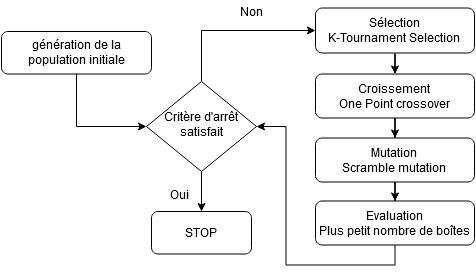
\includegraphics[scale=0.6]{./figures/AG schema.png}
    \caption{Processus de AG }
    \label{fig:agschema}
\end{figure}
Les algorithmes génétiques sont connus par leur Rapidité et facilité d’utilisation. 
En effet, le AG est parmis les métaheuristiques les plus rapides, de plus, si la la représentation vectorielle de l'individu est correcte, nous pouvons trouver une solution sans un travail d'analyse approfondi. Par contre, cette métaheuristique ne trouve pas toujours l’optimum et peut se retrouver avec le problème d’optimum local. 

\subsection{Le Recuit Simulé (SA)}
Le recuit simulé est un algorithme de recherche locale initialement introduit par Kirkpatrick et al \cite{kirk} qui simule la fusion et le refroidissement dans le traitement des métaux. Le recuit simulé est généralement implémenté pour rechercher une solution optimale sur une petite zone, même s'il est parfois aussi performant que AG dans certains cas \cite{Alkhateeb}.
Cette métaheuristique sophistiquée empêche d'être piégé dans les minima locaux à l'aide d'un moteur de recherche aléatoire exprimé en termes de chaîne de Markov. Elle introduit des changements dans la solution pour améliorer la fonction objectif, mais conserve également des solutions qui, malgré les moins bonnes performances, répondent à certains critères. Mais l’un des inconvénients du recuit simulé est son temps d'exécution élevé. 

\subsection{Hybridation et travaux relatifs}
Pour surmonter les inconvénients  de GA et SA, plusieurs études proposent une hybridation entre les deux.
Junghans et Darde \cite{Junghans} comparent entre AG et AG hybride avec SA modifiée (MSA).
 Le SA utilisé dans leur expérience a été modifié pour contrôler la réduction de la température.
 Ils ont découvert que le GA-MSA hybride offre une fiabilité plus élevée que le AG.
 Une autre recherche menée par Chen et Shahandashti dans \cite{Chen} qui compare également le GA, SA, un hybride de GA-SA et MSA, où ils ont constaté que le GA-SA hybride est plus performante que AG, SA et MSA. \\
Dans cet article, nous avons hybridé le GA-SA avec quatres scénarios, à savoir le AG-RS hybride, le AGH-RS, le AG-2RS et le AG-MIX, Le schéma hybride AG-RS consiste à obtenir la meilleure solution en AG et à l'utiliser comme population initiale en SA,
le AGH-RS utilise le même processus sauf que AG à été initialisé par plusieurs heuristiques.Le schema AG-2RS  consiste à inclure SA dans le AG après l’étape de mutation, et améliorer la solution de AG par le SA à nouveau. finalement le schéma AG-MIX utilise le même processus que AG-2RS en initialisant le AG par plusieurs heuristiques. 
D’autres schémas ont été implémenté et serons inclus dans la comparaison, on cite le WOA-RS  et le ILWOA-RS qui sont une hybridation de haut niveau des métaheuristiques WOA\cite{WOA} et ILWOA\cite{ILWOA} avec le recuit simulé.

 
 \subsection{Organisation du papier}
 On va tout d’abord donner la formulation mathématique du problème, par la suite on présentera nos schémas hybrides proposés. Finalement, des résultats expérimentaux sont donnés et une comparaison des schémas hybrides est effectuée  dans (4) , suivi d’une conclusion.

\section{Formulation du problème}
\subsection{Formulation mathématique}
Etant donné \(m\) boites de capacité \(C\) et \(n\) articles de volume \(v_i\) chacun. \\
    Soient: 
    \[ x_{ij} =
        \begin{cases}
            1  & \quad \text{article } j \text{ rangé dans la boîte } i \\
            0  & \quad \text{sinon } 
        \end{cases}
    \]
    \[ y_i =
    \begin{cases}
        1  & \quad \text{boîte } i \text{ utilisée } \\
        0  & \quad \text{sinon } 
    \end{cases}
    \]

La formulation du problème donne ainsi le programme linéaire suivant
\[(PN)
    \begin{cases}
        Z(min) = \displaystyle\sum_{i=1}^{m} y_i \\
        \displaystyle\sum_{i=1}^{m} x_{ij}  = 1 \\
        \displaystyle\sum_{j=1}^{n} v_j x_{ij} \le C y_i \\
        y_i \in \{0,1\} \\
        x_{ij} \in \{0,1\} 
    \end{cases}
\]  
La première contrainte signifie qu’un article j ne peut être placé qu’en une seule boite
La deuxième fait qu’on ne dépasse pas la taille d’une boite lors du rangement

\section{L'approche hybride proposée}
Pour le schéma de l’hybridation proposé dans cet article, il s’agit d’une hybridation classifiée selon la taxonomie de talbi\cite{talbi2002taxonomy} comme suit 
\textbf{HRH globale, généraliste }, et qui utilise l'algorithme génétique comme méthode révolutionnaire,
suivie par un  Recuit Simulé pour l'intensification des résultats de ce dernier.

\subsection{Encodage de la solution}
\subsubsection{Solution du bin packing}
La solution sera représentée par: 
\begin{itemize}
    \item une liste de boîtes, où la boîte est représentée par une liste des objets qui y sont rangés, et l’objet est représenté par un entier désignant son poids.
    \begin{figure}[h!]
        \centering
        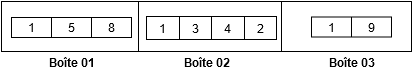
\includegraphics[scale=0.6]{./figures/Untitled Diagram(6).png}
    \end{figure}
    \item Le nombre de boîtes utilisées, ce qui représente le coût de la solution, et nous permettra  d’évaluer la performance de l’algorithme en terme de la qualité de la solution.

\end{itemize}
\subsubsection{Représentation chromosomique}
Pour cette implémentation de l’AG, nous allons utiliser une nouvelle représentation chromosomique, proposée dans \cite{Mohamadi}, On représente une solution du Bin packing comme suit: 
\begin{itemize}
    \item [-]On suppose qu'on a \emph{n} objets à ranger donc on utilisera \emph{n} boîtes au maximum.
    \item [-]Chaque boîte est composée de  \emph{n} cellules, où chaque cellule ne peut contenir qu’un seul objet.
    \item [-]Chaque cellule a un numéro unique dans la solution.
    \item [-]Si la cellule de l'ordre \emph{i} de la boite \emph{j} est remplie par un objet, alors on aura plus le droit de ranger un objet dans toutes les cellules de l’ordre \emph{i} des autres boites.
    \item [-]La cellule \emph{0} contient le nombre de boîtes utilisées dans cette solution.
\end{itemize}
Dans le chromosome , on ne garde trace que des numéros de cellules où les objets sont stockés, donc la taille du chromosome sera de \emph{n+1}.

\subsection{L'hybridation AG-RS}
Une hybridation entre AG et RS permet à AG d'explorer un énorme espace de recherche et à RS d'exploiter des zones de recherche locales. Le RS commence généralement par une solution initiale aléatoire, dans la solution proposée, la meilleure solution de AG est utilisée comme configuration initiale, et le Recuit simulé va se charger de l’intensification de cette dernière, où il utilise un processus de recherche d'une solution optimale globale dans l'espace de la solution, grâce à son aspect aléatoire, et qui a été prouvé de guider l’algorithme vers l’optimum global. 
Donc, le AG est puissant pour obtenir une solution presque optimale sur la zone de recherche large tandis que RS est utile pour rechercher une solution dans la zone de recherche étroite.\cite{Gusti}

\section{Tests et résultats}
Les différents algorithmes ont été développés en utilisant python, et exécutés sur un DELL Inspiron15 [Intel® Core™ i7-8550U CPU @ 1.80GHz×8, 8Go] en utilisant Visual Studio Code. \\
les tests ont été effectué sur le benchmark Scholl \cite{Scholl}, en prenant des instances de petites, moyenne, et grandes taille, ont utilisera par la suite l’encodage suivant 
\begin{table}[h]
\centering
\begin{tabular}{l l l l l l}
\hline
\textbf{Code} & \textbf{N1} & \textbf{N2} & \textbf{N3} & \textbf{N4} & \textbf{HARD} \\
\hline
Valeur  & 50 & 120 & 200 & 500 & HARD \\
\hline
\end{tabular}
\caption{encodage des instances}
\end{table}

\subsection{Calibrage des paramètres}
Les paramètres des métaheuristiques utilisées dans cette article (AG, WOA, ILWOA) ont été fixé en utilisant un outil de calibrage automatique Irace , son implémentation est disponible dans un package R au près de CRAN dans \cite{irace}, ce package implémente une extension de la course F itérée (I / F-Race) expliquée dans \cite{survey}. 
Les configurations optimales des paramètres sont données dans le tableau suivant :\\


\begin{tabular}{l|l|l}
    \hline
    \textbf{Méthode} & \textbf{Paramètre} & \textbf{Valeur}  \\
    \hline
    \textbf{AG} & le nombre de populations générées (nbrGen) & 200 \\ \cline{2-3}
      &paramètre de "k-tournament selection” (k) & 20 \\ \cline{2-3}
      &taille d’une population (popSize) & 10 \\ \cline{2-3}
      &probabilité de croisement & 0.85 \\ \cline{2-3}
      &probabilité de mutation & 0.1\\
    \hline
    \textbf{RS} & le nombre d'itérations (R) & 1000 \\ \cline{2-3}
      & Le facteur de diminution de la température ($\alpha $) & 0.925 \\ \cline{2-3}
    \hline
    \textbf{WOA} & taille de la population (nb-whales) & 30 \\ \cline{2-3}
      & nombre d’itérations (max-iter) & 117 \\ \cline{2-3}
      & constante de l’encerclement spirale (b) & 8.96 \\ \cline{2-3}
      & constante d’exploration (a) & 10 \\ \cline{2-3}
    \hline
    \textbf{ILWOA} & taille de la population (nb-whales) & 10 \\ \cline{2-3}
    & nombre d’itérations (max-iter) & 30(hard),10 \\ \cline{2-3}
    & constante de l’encerclement spirale (b) & 1.5 \\ \cline{2-3}
    & constante d’exploration (a) & 2 \\ \cline{2-3}
    & beta & 1.5 \\ \cline{2-3}
  \hline

\end{tabular}


\subsection{Etude des performances}
Dans le tableau suivant on donne le temps d'exécution moyen de AG-RS en fonction de la taille de l’instance ainsi que l’écart par rapport à solution optimale  en séparant la classe difficile (HARD) dans ce cas. 
\begin{table}[h]
    \centering
    \begin{tabular}{l l l}
    \hline
    \textbf{N/Instances} & \textbf{Temps d'execution (s)} & \textbf{Ecart(\%)} \\
    \hline
    N1=50  & 1.216188 & 0.606618  \\
    \hline
    N2=120  & 3.213707 & 0.446429  \\
    \hline
    N3=200  & 12.083458 & 0.071839  \\
    \hline
    N4=500  & 47.665262 & 1.320662  \\
    \hline
    HARD  &  & 6.059809 \\
    \end{tabular}
    \caption{temps d'execution et écart de AG-RS}
\end{table}


Le temps d'exécution de AG-RS augmente avec la taille de l’instance,  on  voit un plus grand écart au niveau de N4 =500, où le temps moyen de résolution d’une instance est de 48 secondes, qui reste toujours un temps acceptable. Le AG-RS converge vers la solution assez rapidement. \\
Pour toutes les instances du benchmark, AG-RS arrive à donner des solutions très proches des solutions optimales avec un écart qui ne dépasse pas 2\%, sauf le cas des instances  HARD (classe 3) où il atteint une valeur de 6\%.
\subsection{Etude comparative}
Dans cette partie nous allons comparer AG-RS avec d’autres algorithmes de résolution  implémentés , dont les trois autres schémas à base de AG (AGH-RS,AG-MIX-RS, AG-RS2) présentés dans [num section hybridation de l’intro], ainsi que deux autres schémas HRH, HRH-WOA-RS, HRH-ILWOA-RS, utilisant les métaheuristiques WOA[1], ILWOA[2] respectivement, suivi du recuit simulé. la comparaison va inclure les métaheuristiques utilisées ainsi que l’heuristique FF qui est la plus performante parmis les heuristiques du bin packing. 
\newline Les figure 1 et 2 représentent le temps d'exécution et l’écart à la solution optimale en \% (resp) pour chaque méthode implémentée,  en fonction de la taille de l’instance et sa difficulté. 

\begin{figure}[H]
    \centering
    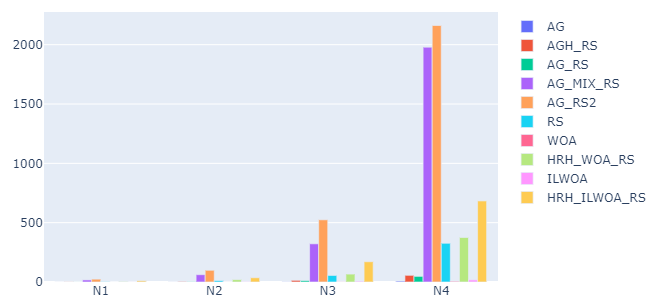
\includegraphics[scale=0.6]{./figures/texec (2).png}
    \caption{Temps d'execution moyen en fonction des tailles d'instances}
\end{figure}

\begin{figure}[H]
    \centering
    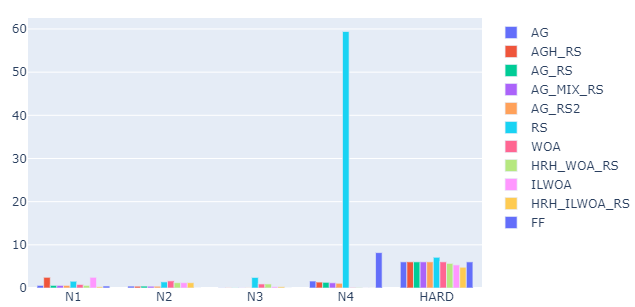
\includegraphics[scale=0.6]{./figures/ecart (2).png}
    \caption{Ecart en \% en fonction des tailles d'instances}
\end{figure}

A partir des deux graphes, on voit que l’algorithme AG-RS permet d’avoir une bonne qualité de solution en un temps d’exécution assez rapide. Il est à noter que les schémas à base de WOA et son amélioration ILWOA permettent d’avoir une légère amélioration de la qualité de solution pour les instances difficiles (HARD), cependant la lenteur de leur exécution les rend moins intéressants.
 Les schémas où les heuristiques sont utilisées dans l’initialisation de AG (AGH-RS, AG-MIX-RS) ont une qualité dégradée par rapport à leurs versions sans heuristiques (AG-RS , AG-2RS resp),
  on justifie ce résultat par leur coincement dans un optimum local, en effet une meilleure amélioration est d’utiliser les heuristiques dans l’initialisation d’une petite partie de la population et garder l’aspect aléatoire dans le reste pour éviter ce problème. Il est clair que le recuit simulé consomme un temps d'exécution très grand, mais offre une qualité de solution très bonne,
   sauf dans le cas N4 où un écart de 60\% est trouvé, ceci est dû à la limite de temps imposée dans l'implémentation de l’algorithme, qui n’as pas permi à RS d’explorer correctement le voisinage. 
   Les schémas utilisant le RS dans chaque itération de AG ( AG-2RS, AG-MIX-RS) ont un temps d'exécution inacceptable avec l’une des meilleures qualités de solutions (AG-2RS) , une meilleure version est d'utiliser une recherche locale moins sophistiqué que RS et l’appliquer chaque lot d’itération.
    Finalement, l’heuristique FF donne une qualité assez bonne dans les instances de petites taille (N1,N2) avec un temps d'exécution négligeable, l’apport des MH et l’hybridation est plus visible et intéressant à partir des instances moyenne et grande taille. 

\section{Conclusion}
Dans cet article, on s’est intéressé au problème du bin packing, où on a proposé un schéma hybride AG-RS. Pour montrer les performances de cet algorithme, on l’a comparé avec d’autres schémas proposées à base des métaheuristiques AG, WOA, et ILWOA. Les tests ont été effectué sur le benchmark scholl et les résultats ont été donné en temps d'exécution moyen et écart à la solution optimale. Notre schéma AG-RS est celui qui assure un bon compromis qualité coût. Pour pousser l’étude, on propose l’utilisation d’une heuristique de recherche locale dans quelques itérations de AG et ILWOA. 
\medskip

\bibliography{Samples}

\end{document}
